\documentclass[Times, 10]{beamer}

\renewcommand{\figurename}{}
\usepackage[font={footnotesize,it}]{caption}
%
\usepackage{amssymb,latexsym,amssymb,amsmath,amsbsy,amsopn,amstext,upgreek}
\usepackage{color,multicol}
\usepackage{graphicx,wrapfig,fancybox,watermark,graphics}
\usepackage{picins}
%\usepackage{pgf}
%\usepackage{media9}
\usepackage{hyperref}
\hypersetup{
    pdfpagemode=FullScreen, % show in full screen?
}
\usepackage{pdfpages}

\usepackage{listings,bera}
\definecolor{keywords}{RGB}{255,0,90}
\definecolor{comments}{RGB}{60,179,113}
\lstset{language=C,
    keywordstyle=\color{keywords},
    commentstyle=\color{comments}\emph
}
\usepackage{algorithm}
\usepackage{algorithmic}
\renewcommand{\algorithmicrequire}{\textbf{Input:}}
\renewcommand{\algorithmicensure}{\textbf{Output:}}

% set fonts
%% \usepackage{fontspec}
%% %\setsansfont{Fontin Sans}
%% \setsansfont{Times}
%% \setbeamerfont{frametitle}{size=\LARGE,series=\bfseries}

%% \usepackage{xeCJK}
%% \usepackage{xltxtra}
%% %       beamer
%% % \usefonttheme{default} % sans serif
%% \usefonttheme{professionalfonts}
%% \usefonttheme{serif}

% reference entry
\usepackage{bibentry}
\usepackage[numbers]{natbib}

\usepackage[
    compress,
    %minimal,
    nonav,
    %red,
    %gold,
    blue,
    numbers,
    nologo,
    %polyu,
    comp,
    forty,
    %seventyfive,
]
{beamerthemeHongKong}

%
\usepackage{graphicx} % graphics
\usepackage{epsfig} % eps graphics
\usepackage{hyperref} % urls
\usepackage{booktabs, caption} % table styling

% suppress navigation bar
\beamertemplatenavigationsymbolsempty

%% \mode<presentation>
%% {
%%   \usetheme{bunsen}
%%   \setbeamercovered{transparent}
%%   \setbeamertemplate{items}[circle]
%% }

\mode<presentation>
{
%  \usetheme{Warsaw}
\usetheme{bunsen}       
  \setbeamercovered{transparent}
  \setbeamertemplate{items}[ball]
  \setbeamertemplate{theorems}[numbered]
  \setbeamertemplate{footline}[frame number]
}

% set fonts
\usepackage{fontspec}
%\setsansfont{Fontin Sans}
\setsansfont{Times}
\setbeamerfont{frametitle}{series=\bfseries} %size=\LARGE

% color definitions
\usepackage{color}
\definecolor{uipoppy}{RGB}{225, 64, 5}
\definecolor{uipaleblue}{RGB}{96,123,139}
\definecolor{uiblack}{RGB}{0, 0, 0}

% caption styling
\DeclareCaptionFont{uiblack}{\color{uiblack}}
\DeclareCaptionFont{uipoppy}{\color{uipoppy}}
\captionsetup{labelfont={uipoppy},textfont=uiblack}


%----------------------------------------
% see the macros.tex file for definitions
%\include{macros}
%---------------------------------

% adds reference to bottom right of corner of a slide
%% \usepackage[absolute,overlay]{textpos} % text references in slide corners
%% \newcommand\textref[1]{%
%%   \begin{textblock*}{\paperwidth}(0pt,0.99\textheight)
%%   \raggedleft \tiny{\emph{#1}}\hspace{.5em}
%%   \end{textblock*}}

% for drawing circles around numbers
% ex. \circled{1} Add some text here.
\usepackage{tikz}
\newcommand*\circled[1]{\tikz[baseline=(char.base)]{
            \node[shape=circle,draw,inner sep=2pt] (char) {#1};}}

%%--------
%\documentclass[11]{beamer}
\setbeamertemplate{navigation symbols}{}

\usepackage{beamerthemeshadow}
 

\usecolortheme[named=blue]{structure}

\mode<presentation>
{
  \usetheme{Warsaw}
  \setbeamercovered{transparent}
  \setbeamertemplate{items}[ball]
  \setbeamertemplate{theorems}[numbered]
  \setbeamertemplate{footline}[frame number]
}

% set fonts
\usepackage{fontspec}
%\setsansfont{Fontin Sans}
\setsansfont{Times}
\setbeamerfont{frametitle}{series=\bfseries} %size=\LARGE

 
%\usepackage{beamerthemeintridea}
 \usepackage{beamerthemesplit}
% \usetheme{Berkeley}
% \usetheme{Warsaw}
% \usecolortheme{dolphin}

%\usepackage{beamerthemesplit}
\usepackage{graphics}
\usepackage{graphicx}
\usepackage{hyperref}



\usepackage{graphicx} % graphics
\usepackage{epsfig} % eps graphics
\usepackage{hyperref} % urls
\usepackage{booktabs, caption} % table styling

%% % suppress navigation bar
%\beamertemplatenavigationsymbolsempty

\mode<presentation>
{
  \usetheme{bunsen}
  \setbeamercovered{transparent}
  \setbeamertemplate{items}[circle]
  \setbeamertemplate{footline}[frame number]
}

%% % set fonts
\usepackage{fontspec}
%\setsansfont{Fontin Sans}
\setsansfont{Times}
\setbeamerfont{frametitle}{series=\bfseries} %size=\LARGE

%% % color definitions
\usepackage{color}
\definecolor{uipoppy}{RGB}{225, 64, 5}
\definecolor{uipaleblue}{RGB}{96,123,139}
\definecolor{uiblack}{RGB}{0, 0, 0}

%% % caption styling
\DeclareCaptionFont{uiblack}{\color{uiblack}}
\DeclareCaptionFont{uipoppy}{\color{uipoppy}}
\captionsetup{labelfont={uipoppy},textfont=uiblack}


%----------------------------------------
% see the macros.tex file for definitions
%\include{macros}
%---------------------------------

% adds reference to bottom right of corner of a slide
%% \usepackage[absolute,overlay]{textpos} % text references in slide corners
%% \newcommand\textref[1]{%
%%   \begin{textblock*}{\paperwidth}(0pt,0.99\textheight)
%%   \raggedleft \tiny{\emph{#1}}\hspace{.5em}
%%   \end{textblock*}}

%% % for drawing circles around numbers
%% % ex. \circled{1} Add some text here.
\usepackage{tikz}
\newcommand*\circled[1]{\tikz[baseline=(char.base)]{
            \node[shape=circle,draw,inner sep=2pt] (char) {#1};}}


%% %------------------------------------
%% %----------------------

\usepackage{amssymb,latexsym,amssymb,amsmath,amsbsy,amsopn,amstext,upgreek}
\usepackage{color,multicol}
\usepackage{graphicx,wrapfig,fancybox,watermark,graphics}
\usepackage{picins}
\usepackage{pgf}
%\usepackage{media9}
\usepackage{hyperref}
\hypersetup{
%    pdfpagemode=FullScreen, % show in full screen?
}
\usepackage{pdfpages}

\usepackage{listings,bera}
\definecolor{keywords}{RGB}{255,0,90}
\definecolor{comments}{RGB}{60,179,113}
\lstset{language=C,
    keywordstyle=\color{keywords},
    commentstyle=\color{comments}\emph
}
\usepackage{algorithm}
\usepackage{algorithmic}
\renewcommand{\algorithmicrequire}{\textbf{Input:}}
\renewcommand{\algorithmicensure}{\textbf{Output:}}

% reference entry
\usepackage{bibentry}
\usepackage[numbers]{natbib}

\usepackage[
    %compress,
    minimal,
    %nonav,
    %red,
    %gold,
    blue,
    %numbers,
    nologo,
    polyu,
    comp,
    forty,
    seventyfive,
    ]{beamerthemeHongKong} 
    
%{beamerthemePittsburgh}
% {beamerthemeAnnArbor}



%========================================

%----------------------
%----------------------

\usepackage{fontspec}
\setsansfont{Courier}
%\setsansfont{Times}
%\setbeamerfont{frametitle}{series=\bfseries} %size=\LARGE




\newcommand{\figdir}[1]{figures/#1}
\newcommand{\figdirTwo}[1]{figures/#1}
\newcommand{\subdir}{}
\newcommand{\subdirTwo}{figures_fullsky/l105mpow2ns1024/}
\newcommand{\subdirThree}{figures_fullsky/l105mpow3ns1024/}
\newcommand{\subdirGal}{figures_galactic80/l105mpow1ns1024/}
\newcommand{\subdirPl}{figures_planck/l105mpow1ns1024/}


\newcommand{\subdirj}{figures_fullsky/mpow1j10beta2048/}
\newcommand{\subdirjTwo}{figures_fullsky/mpow2j10beta2048/}
\newcommand{\subdirjThree}{figures_fullsky/mpow3j10beta2048/}
\newcommand{\subdirGalj}{figures_galactic80/mpow1j10beta2048/}
\newcommand{\subdirPlj}{figures_planck/mpow1j10beta2048/}

\newcommand{\figmask}[1]{/Users/yabebal/My-Works/planck/mf_paper1_output/masks/#1}


\newcommand{\figref}[1]{Figure (\ref{#1})}
%\newcommand{\eqref}[1]{Eqn. (\ref{#1})}
\newcommand{\reffig}[1]{Figure (\ref{#1})}
\newcommand{\refeq}[1]{Eqn. (\ref{#1})}
\newcommand{\refsec}[1]{Section \ref{#1}}
\newcommand{\healpix}{HEALpix~}
\newcommand{\nside}[1]{N_{\rm side}}


\title{{Application of the second order Gaussian kinematic formula to CMB
    data analysis}}
  

\author{Yabebal Fantaye}
\institute[Cape Town]{
  { African Institute For Mathematical Sciences (AIMS) \\
    South Africa} \\ 
\inst{} \\
 In collaboration with: D. Marinucci, V. Cammarota}


\date{\today} 

% \pgfdeclaremask{uio}{uio}
% \pgfdeclareimage[mask=fsu,width=1cm]{fsu-logo}{uio}
% 
% \logo{\vbox{\vskip0.1cm\hbox{\pgfuseimage{f/mn/stornext/u2/yabebalf/My-Works/Writings/kile-LocEnv/uio_logo_ny.pdf}}}}

\begin{document}



 % \setbeamertemplate{background}
 % {\includegraphics[width=\paperwidth,height=\paperheight]{frontpage_bg}}
 % \setbeamertemplate{footline}[default]

%% \begin{frame}
%% \vspace{2cm}
%% \begin{columns}
%% \column{2.75in}
%%   \titlepage
%%   \vspace{10cm}
%% \column{2.0in}
%% \end{columns}
%% \end{frame}



%-----------------------------------------------------------------------------80
  \frame
  {
    \titlepage
  }


%-------------------------------------------------------------------
%                          Section 1
%-------------------------------------------------------------------
%
% Set the background for the rest of the slides.
% Insert infoline
%% \setbeamertemplate{background}
%%  {\includegraphics[width=\paperwidth,height=\paperheight]{slide_bg}}
%% \setbeamertemplate{footline}[bunsentheme]


%-----------------------------------------------------------------------------80
   \section*{Outline}
% %-----------------------------------------------------------------------------80
  \frame
  {
    \frametitle{Outline}

    \tableofcontents
  }


%-----------------------------------------------------------------------------80
\section{Introduction}
%-----------------------------------------------------------------------------80

\frame {
\frametitle{Geometry of Gaussian Random Fields}

\begin{itemize}

\item Let $M$ be a general Riemannian manifold. In particular, for CMB we can think of $M$ as a sphere $S^2$.
\item  The basic set of random geometrical objects are $\mathcal{R}$ valued random field $f(x)$ defined on M and its excursion sets $A$ 

\[
A_u(f, M) = \{ x \in M : f(x) \geq u \} 
\] 

%\item our interest here is to study the geometry e.g. peaks, isocontour lengths, area of these objects 

\end{itemize}

\begin{figure}
\begin{center}
\includegraphics[width=0.33\textwidth,angle=0]{\figdirTwo{map_sup_u-3_fwhm5deg.pdf}} 
\includegraphics[width=0.33\textwidth,angle=0]{\figdirTwo{map_sup_u-2_fwhm5deg.pdf}} 
\includegraphics[width=0.33\textwidth,angle=0]{\figdirTwo{map_sup_u-1_fwhm5deg.pdf}} \\ 
\includegraphics[width=0.33\textwidth,angle=0]{\figdirTwo{map_sup_u0_fwhm5deg.pdf}} 
\includegraphics[width=0.33\textwidth,angle=0]{\figdirTwo{map_sup_u1_fwhm5deg.pdf}} 
\includegraphics[width=0.33\textwidth,angle=0]{\figdirTwo{map_sup_u2_fwhm5deg.pdf}} 
%\includegraphics[width=0.33\textwidth,angle=0]{\figdirTwo{map_sup_u3_fwhm5deg.pdf}} 
\end{center}
\end{figure}



}

%----------------------------------------------
\frame {

  \frametitle{Morphological Properties}
  Morphological properties are the characteristics of the field which are
  invariant under translations and rotations and which are additive
  i.e the Minkowski Functionals -  Area, Perimeter Length and Euler Poincar\'e characteristics

}

  \theorem{Hadwiger Theorem (1959)}{all properties of a
d-dimensional convex set (or more generally, a finite union of convex
sets) which satisfy the morphological properties are contained in d + 1 MF values.}

Note that for a digital image, one can consider a pixel as a compact and convex set.

\frame {

  \frametitle{Minkowski Functionals Properties}


For $\mathca{K}^d$ the class of convex, compact sets in $\mathca{R}^d$, a continuous map $T : \mathca{K}^d \rightarrow \mathcal{R}$
\begin{equation}
T(gK)=T(K) \forall{K}\in \math{K}^d, g\in G_d  
\end{equation}

where $G_d$ is the group of rigid motions in $d$ dimensions (i.e.
rotations and translations); and 

\begin{equation}
T(K_1 \intersection K_2) + T(K_1 \union
K_2) = T(K_1) + T(K_2)
\end{equation}
for $K_1,K_2\in \mathca{K}^n$
with $K_1 \intersection K_2 \in \mathca{K}^d$. Then
$T$ can be expressed as a linear combination of the MFs

\begin{equation}
  T(K) = \sum_{i=0}^{d}\alpha_i W_i(K) \hspace{1cm} \alpha_i\in \mathcal{R}
\end{equations}
 
}

\frame {

  \frametitle{Steiner formula}

  \begin{equation}
    W_j(K_r) = \sum_{i=0}^{d-j}{d-j}\choose{i}W_{i+j}(K)r^i
  \end{equation}

  The generalized Steiner formula can also be generalized to the other Minkowski functionals besides volume as
}
  
  % ----------------------------------------------

\frame {

  \frametitle{Lifschitz-Killing Curvatures (Minkowski Functionals)}

  \begin{itemize} 

    \item Lifschitz-Killing Curvatures (LKCs), a.k.a Minkowski Functionals (MFs), can be defined using a tube formula:
    
    \[
    \mu(Tube(M,\rho)) = \sum_{j=0}^{n=dim(M)}{\omega_j\mathcal{L}_{n-j}(M)\rho^j}
    \]

    where $Tube(M,\rho) = \{ t\in \mathcal{R}^N : dist(M,x)\leq\rho \}$ is a
    tube of radius $\rho$ bounding M; $\mu$ is Lebesgue measure; and
    $w_j$ is the volume of a unit ball in $\mathcal{R}^j$.
    
  \item LKCs depend on the Riemannian metric, and are a measure of the k-dimensional size of the
    Riemannian manifold $M$.

  %% \item For example in $n=2$, $\mathcal{L}_{0}$ corresponds to the
  %%   genus ; $\mathcal{L}_{1}$ to the perimeter/2 and
  %%   $\mathcal{L}_{2}(M)$ to the area.
    
  \end{itemize}

}

%-----------------------------------------------------------------------------

\frame {
  
  \frametitle{Lifschitz-Killing Curvatures (Minkowski Functionals) II}   
    \begin{itemize}
    \item $\mathcal{L}_{0}(A_{u}(f))$ is the genus or the
      Euler-Poincar\`{e} characteristic (minima+maxima-saddles) of the
      excursion regions. The third Minkowski functional. \\
    \item $\mathcal{L}_{1}(A_{u}(f))$ is half the boundary length of
      the excursion regions, e.g. the second Minkowski functional. \\
    \item $\mathcal{L}_{2}(A_{u}(f))$ is the area of the excursion
      regions, e.g.  the first Minkowski functional.
    \end{itemize}
    
    
  }

%-----------------------------------------------------------------------------80
\section{The Gaussian Kinematic Formula (GKF)}
%-----------------------------------------
\frame {
  
  \frametitle{The Gaussian Kinematic Formula (GKF) }
  
  \begin{itemize}

  \item Developed by Adler \& Taylor, it is about expected
    values of Lifshitz-Killing curvatures (LKCs)/Minkowski Functionals
    (MFs) for excursion regions.

  %% \[
  %% A_{u}(f):=\left\{ x\in S^{2}:f(x)\geq u\right\} \text{ .} 
  %% \]%
  
    \[
    \mathbb{E}\mathcal{L}_{i}(A_{u}(f,M))=\sum_{k=0}^{dim M - i}{i+k \brack k}
           {\mathcal{L}_{i+k}}(M)\mathcal{M}_{k}([u,\infty))
             \]
           
           {\small
             
             where
             \[
               {i+k \brack k} = {i+k \choose k}\frac{\omega_{i+k}}{\omega_k\omega_i}  
               \]
           }
           
         \item $\mathcal{M}$ is given by
           {\small
             \[
             \mathcal{M}_j^{\gamma_k}([u,\infty))=(2\pi)^{-1/2}H_{j-1}(u)e^{-u^2/2}.
               \]
             }
             
             where $H_j$ is the Hermite polynomials: $H_0(u)=1$, $H_1(u)=2u$, $H_2(u)=4u^2-1$, $H_3(u)=8u^3-12u$ 
  \end{itemize}
}

 

%-----------------------------------------------------------------------------80


\frame {

  \frametitle{The power of GKF }
  \begin{itemize}
  \item Splits the metric dependence of the field from that of excursion set behaviour.
  \item The $\mathcal{L}_{k}(M)$ part contains all the metric property. If
    the metric is scaled by $\lambda$, $\mathcal{L}_{k}(M)$ scales by
    $\lambda^k$. 


  \item  On a sphere the scaling $\lambda$ required to go to harmonic space is given by:
    \[
      \lambda_{s}= \sqrt{\frac{s(s+1)}{2}}, & \text{if } f(x)=T_\ell(x) \\
    \]
    
  %% \item On a sphere $S^2$ with a given basis i.e harmonic or needlet,
  %%   we can write 

%% where  and possible boundaries i.e cut-sky
%%     \[
%%     \mathcal{L}_{0}(M)=2\text{ , }\mathcal{L}_{1}(M)=\frac{1}{2}\text{boundary
%%       length},\text{ }\mathcal{L}_{2}(M)=f_{sky}4\pi \text{ ,}
%%     \]%
    
   
      
     %  \[
     %  \lambda_{s}= \begin{cases} 
     %    \sqrt{\frac{s(s+1)}{2}}, & \text{if } f(x)=T_\ell(x) \\ 
     %    \sqrt{\frac{ \sum_{\ell} b^{2}(\frac{\ell}{2^{s}})C_{\ell}\frac{2\ell+1}{4\pi}\frac{\ell(\ell+1)}{2}}%
     %         {\sum_{\ell} b^{2}(\frac{\ell}{2^{s}})C_{\ell}\frac{2\ell+1}{4\pi}}},
     %         & \text{if }f(x) = \beta_{j}(x)
     %  \end{cases}       
     % \]

  \item The $\mathcal{M}_{k}([u,\infty))$ part dependence only on the
    excursion threshold $u$. It absorbs all non-linear transformations:
      \[
      H_{ns}(x):=H_{n}(f(x))=\frac{f^{n}(x)}{\sum_{l}b^{2}(\frac{%
          l}{B^{s}})\frac{2l+1}{4\pi }C_{l}}-1\text{ .} \text{where } n=2,3,..
      \]



  \end{itemize}
  

  }

%--------------------------------------------------------

%------------------------------------
\section{Applications of GKF in cosmology}
%------------------------------------

\frame {

\frametitle{Applications of GKF in cosmology}

\begin{itemize}

\item Our interest here is to compute the expected values of the LKCs
  (MFs) in harmonic and needlet space.

\item The advantages of implementing LKCs on needlet space are:

\begin{itemize}
\item Needlets enjoy very good localization in pixel space - are
  minimally affected by masked regions, especially at high-frequency
  $j.$

\item The double-localization properties of needlets (in real and harmonic
space) allow a precise interpretation of any possible anomalies - offer a
 scale-by-scale probe of asymmetries and relevant
features e.g. \emph{Cold Spot}. 

%% \item The large low-$\ell$ cosmic variance affects MFs on the
%%   full-sky, while this is not the case for MFs evaluated at the
%%   highest needlet scales. The variance of normalized components may be
%%   shown to decrease steadily, entailing a much greater detection power
%%   in the presence of anomalies.
\end{itemize}

\end{itemize}

}

%------------------------------------------------------

\subsection{Harmonic and needlet space LKCs: Gaussian case}
%-----------------

\frame{
\frametitle{LKCs for a Gaussian field}

\begin{itemize}

\item The expected value of the first Lipschitz-Killing curvature (e.g. Euler-Poincar\`{e} characteristic)
\[
\mathbb{E}\mathcal{L}_{0}(A_{u}(f(x),S^{2}))=2\left\{ 1-\Phi
(u)\right\} + \lambda_{s}^2\frac{ue^{-u^{2}/2}}{\sqrt{(2\pi )^{3}}}4\pi \text{ ;} 
\]

\item The second Lipschitz-Killing curvature (e.g., half the boundary
length) 
\[
\mathbb{E}\mathcal{L}_{1}(A_{u}(f(x),S^{2}))=\pi \times  
\lambda_{s}e^{-u^{2}/2}\text{ ;} 
\]

\item The third Lipschitz-Killing curvature (e.g., the area of the
excursion region)
\[
\mathbb{E}\mathcal{L}_{2}(A_{u}(f(x),S^{2}))=4\pi \times \left\{
1-\Phi (u)\right\} \text{ .} 
\]%


\end{itemize}
}



%---------------------------------------
\section{Simulations}
%-----------------------------------------------------------------------------80

\frame {

  \frametitle{Computing LKCs from a (CMB) map}
  \begin{itemize}     
    \item Harmonic space - obtain $T_\ell(x)$ maps; normalize each map
      by the expected RMS; power transform normalized $T_\ell$ maps to
      obtain NG maps.
  \item Needlet space - apply the standard needlet filter to the
    spherical harmonic coefficients; obtain needlet maps $\beta_j(x)$;
    normalize each map by the expected RMS; power transform normalized
    $\beta_j(x)$ maps to obtain NG maps. The $j^{th}$ needlet map has a
    compact support for $\ell$-range between $B^{j-1}$ and $B^{j+1}$
    where we used B=1.5. \\

  \item The area functional is computed by finding the ratio of
    Healpix pixels above a certain temperature threshold. \\

  \item The length and genus functionals are computed by using the
    method described in Eriksen et. al. 2004 paper.
  \end{itemize}
}


%-----------------------------------------------------------------------------80


\frame{
\frametitle{Multipole space -  Gaussian case}
\begin{figure}[H]
\begin{center}
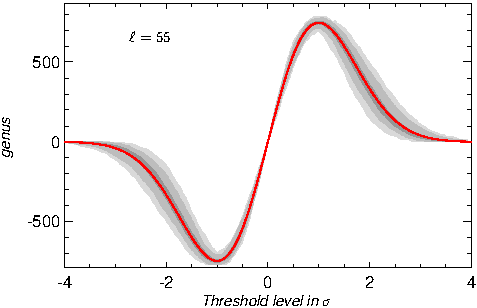
\includegraphics[width=0.31\textwidth,angle=0]{\figdir{\subdir/genus_mpow1_ell_55_compare.pdf}}
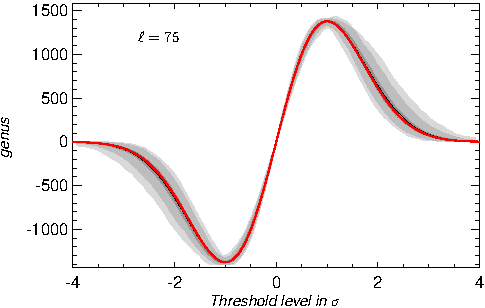
\includegraphics[width=0.31\textwidth,angle=0]{\figdir{\subdir/genus_mpow1_ell_75_compare.pdf}}
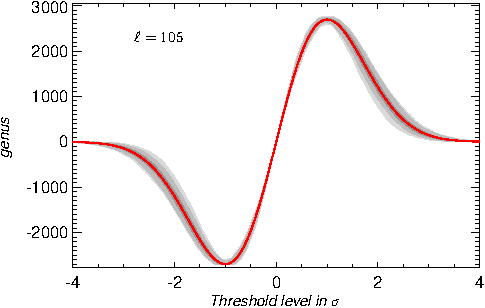
\includegraphics[width=0.31\textwidth,angle=0]{\figdir{\subdir/genus_mpow1_ell_105_compare.pdf}} \\
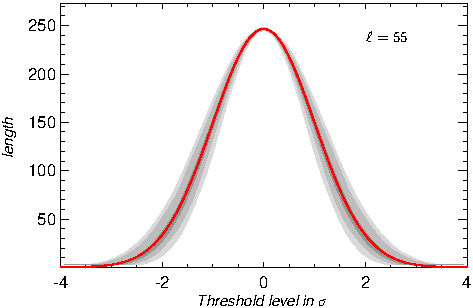
\includegraphics[width=0.31\textwidth,angle=0]{\figdir{\subdir/length_mpow1_ell_55_compare.pdf}}
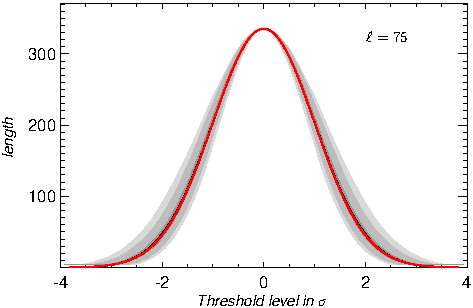
\includegraphics[width=0.31\textwidth,angle=0]{\figdir{\subdir/length_mpow1_ell_75_compare.pdf}}
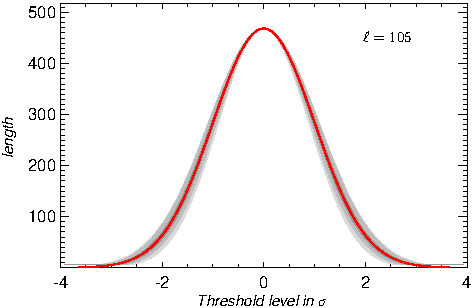
\includegraphics[width=0.31\textwidth,angle=0]{\figdir{\subdir/length_mpow1_ell_105_compare.pdf}} \\
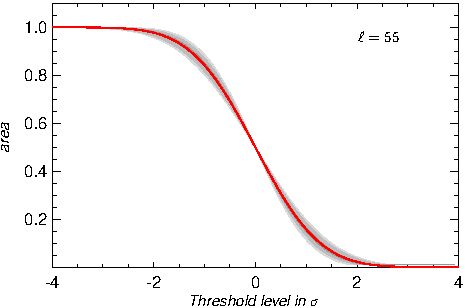
\includegraphics[width=0.31\textwidth,angle=0]{\figdir{\subdir/area_mpow1_ell_55_compare.pdf}}
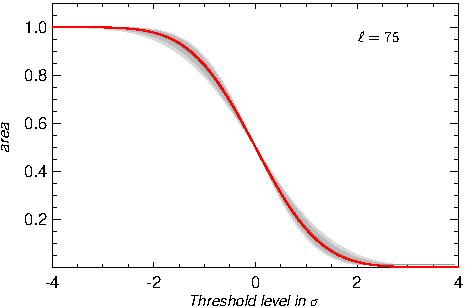
\includegraphics[width=0.31\textwidth,angle=0]{\figdir{\subdir/area_mpow1_ell_75_compare.pdf}}
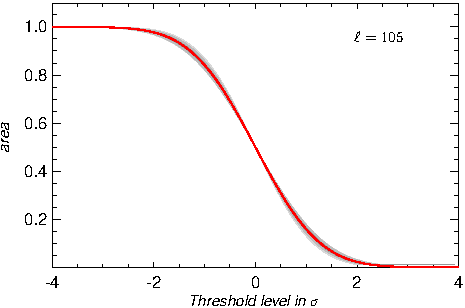
\includegraphics[width=0.31\textwidth,angle=0]{\figdir{\subdir/area_mpow1_ell_105_compare.pdf}} \\
\caption{ Analytical (blue curve) vs Simulation (black and grey. Grey Shades are $68, 95$ and $99
  \%$ percentiles estimated from 100 simulations.}
\end{center}
\end{figure}


}


%--------------------------------------

\section{Summary and Conclusion}
%----------------------------------------
\frame{
\frametitle{Summary}

\begin{itemize}
\item Exact formula on full sky - no flat sky approximation! \\
\item Analytical results agrees very well with simulations.
\item Evaluation in both multipole and needlet space: \\
\begin{itemize}
\item separates scale/frequency \\
\item mitigates contamination of high-frequency modes by the large low-$\ell$  cosmic variances.  \\
\item allows a unified measure of deviation from Gaussianity (work in progress)\\
\end{itemize}
\item Handles effect of mask analytically!! \\
\item Handles non-Gaussianity analytically. \\
\item Analytical predications of the LKCs variances (work in progress).
\end{itemize}

}



%% \frame{

%% \begin{figure}
%% \begin{center}
%% \includegraphics[width=0.31y5\textwidth,angle=0]{\figdirTwo{map_sup_u-2_fwhm1deg.pdf}} 
%% \includegraphics[width=0.33\textwidth,angle=0]{\figdirTwo{map_sup_u-1_fwhm1deg.pdf}} 
%% \includegraphics[width=0.33\textwidth,angle=0]{\figdirTwo{map_sup_u0_fwhm1deg.pdf}} \\
%% \includegraphics[width=0.33\textwidth,angle=0]{\figdirTwo{map_sup_u1_fwhm1deg.pdf}} 
%% \includegraphics[width=0.33\textwidth,angle=0]{\figdirTwo{map_sup_u2_fwhm1deg.pdf}} 
%% \includegraphics[width=0.33\textwidth,angle=0]{\figdirTwo{map_sup_u3_fwhm1deg.pdf}} 
%% \end{center}
%% \end{figure}

%% }

%% \frame{

%% \begin{figure}
%% \begin{center}
%% \includegraphics[width=0.33\textwidth,angle=0]{\figdirTwo{map_sup_u-4_fwhm10deg.pdf}} 
%% \includegraphics[width=0.33\textwidth,angle=0]{\figdirTwo{map_sup_u-2_fwhm10deg.pdf}} 
%% \includegraphics[width=0.33\textwidth,angle=0]{\figdirTwo{map_sup_u0_fwhm10deg.pdf}} \\
%% \includegraphics[width=0.33\textwidth,angle=0]{\figdirTwo{map_sup_u1_fwhm10deg.pdf}} 
%% \includegraphics[width=0.33\textwidth,angle=0]{\figdirTwo{map_sup_u2_fwhm10deg.pdf}} 
%% \includegraphics[width=0.33\textwidth,angle=0]{\figdirTwo{map_sup_u3_fwhm10deg.pdf}} 
%% \end{center}
%% \end{figure}

%% }

%%\item LKCs 
%% \item  the Lebesgue and Gaussian measure of the tube defines the Lifschitz-Killing Curvatures (LKCs) $\mathcal{L}_{k}(M)$ and Gaussian Minkowski Functionals (GMFS) $\mathcal{M}_{dim(M)-k}(M)$ respectively. 


%% \item  Let $\gamma=\gamma_k$ be a Gauss measure on $\mathcal{R}$ so that for $A \subset \mathcal{R}$
%% \[
%% \gamma_k(A) = (2\pi)^{-k/2}\int_A{e^{-|x|^2/2}dx}.
%% \]

%% \item now define a tube around $A$ such that
%%  \[
%%  \gamma_k(Tube(A,\rho)) = \gamma_k(A) + \sum_{j=1}^{\infty}{\frac{\rho^j}{j!}\mathcal{M}_j^{\gamma_k}(A)}
%% \]

%% \item $\mathcal{M}_j^{\gamma_k}(A)$ for $j \geq 1$ are called Gaussian MFs.

%%\item  For example for $[u,\infty)\subset R$

%%\item $\mathcal{M}_1$, $\mathcal{M}_2$, $\mathcal{M}_3$ are known as the \emph{area}, \emph{length} and \emph{genus} respectively.

  %% \item The three Minkowski functionals  (MFs) are: \\
  %%   \begin{itemize} 
  %% \item Area: the fraction of area  above a certain temperature or polarisation intensity threshold \\
  %%  \item Length: the length of the boundary between fractions, below and above a certain threshold.  \\
  %%  \item Genus: Given the number of minima ($N_{min}$), maxima ($N_{max}$) and saddle points ($N_{sadl}$) 
  %%   above a certain threshold, it is defined as G =  $N_{min}+N_{max} - N_{sadl}$ \\
  %%     \end{itemize}

%--------------------------------------------------
%-----------------------------------------------------------------------------80

%% \frame
%% {
%%   \frametitle{Gaussian Minkowski Functionals (MFs)}

%%   \begin{itemize} 
%% \item  Let $\gamma=\gamma_k$ be a Gauss measure on $\mathcal{R}$ so that for $A \subset \mathcal{R}$
%% \[
%% \gamma_k(A) = (2\pi)^{-k/2}\int_A{e^{-|x|^2/2}dx}.
%% \]

%% \item now define a tube around $A$ such that
%%  \[
%%  \gamma_k(Tube(A,\rho)) = \gamma_k(A) + \sum_{j=1}^{\infty}{\frac{\rho^j}{j!}\mathcal{M}_j^{\gamma_k}(A)}
%% \]

%% \item $\mathcal{M}_j^{\gamma_k}(A)$ for $j \geq 1$ are called Gaussian MFs. For example for $[u,\infty)\subset R$
%% \[
%% \mathcal{M}_j^{\gamma_k}([u,\infty))=(2\pi)^{-1/2}H_{j-1}(u)e^{-u^2/2}.
%% \]

%% \item $\mathcal{M}_1$, $\mathcal{M}_2$, $\mathcal{M}_3$ are known as the \emph{area}, \emph{length} and \emph{genus} respectively.

%%   %% \item The three Minkowski functionals  (MFs) are: \\
%%   %%   \begin{itemize} 
%%   %% \item Area: the fraction of area  above a certain temperature or polarisation intensity threshold \\
%%   %%  \item Length: the length of the boundary between fractions, below and above a certain threshold.  \\
%%   %%  \item Genus: Given the number of minima ($N_{min}$), maxima ($N_{max}$) and saddle points ($N_{sadl}$) 
%%   %%   above a certain threshold, it is defined as G =  $N_{min}+N_{max} - N_{sadl}$ \\
%%   %%     \end{itemize}

%%   \end{itemize}

%% }

%-----------------------------------------------------------------------------80

%% \frame {
%%   \frametitle{Lipschitz-Killing curvatures (LKCs)}
  
%%   \begin{itemize} 
%%     \item To be defined
%% \end{itemize}
  
%%   }
  
%-----------------------------------------------------------------------------80

%\frame {

%%     \begin{figure}

%%     \includegraphics[width=0.30\textwidth]{\figdir{asymm_Aps_30_ruler_common_ddx9.png}}
%% \includegraphics[width=0.30\textwidth]{\figdir{asymm_Aps_30_nilc_common_ddx9.png}} 
%% \includegraphics[width=0.30\textwidth]{\figdir{asymm_Aps_30_sevem_common_ddx9.png}} \\
%% \includegraphics[width=0.30\textwidth]{\figdir{asymm_Aps_30_smica_common_ddx9.png}}
%% \includegraphics[width=0.30\textwidth]{\figdir{asymm_Aps_30_smica_smica_ddx9.png}}
%%         \caption{Commander-Ruler, NILC, SEVEM, SMICA, SMICA**}
%%     \end{figure}


%}

\end{document}
